% 页面设置
\documentclass[12pt, a4paper]{article} % 字号:12,纸张:A4
\usepackage[top=2.54cm, bottom=2.54cm, left=3.18cm,right=3.18cm]{geometry} % 页边距设置
% 字体设置
\usepackage[UTF8]{ctex}
\usepackage{fontspec} % 设置字体
%\setCJKmainfont{SimSun}[AutoFakeBold=true, BoldFont={SimHei}, ItalicFont={KaiTi}] % 正文字体
%\setCJKsansfont[AutoFakeBold=3]{KaiTi} % 无衬线字体
%\setCJKmonofont[AutoFakeBold=3]{SimHei} % 等宽字体
\setmainfont{Times New Roman} % 设置主字体为新罗马体
% 文本设置
\usepackage{enumerate} % 支持小标题编号
\linespread{1.5} % 行间距1.5倍
\usepackage{indentfirst}%首段缩进
\setlength{\parindent}{2em} % 首行缩进两字符
\usepackage[hidelinks]{hyperref} % 目录添加超链接
\usepackage{zhnumber} % 章节标题中文显示
\usepackage[cmyk]{xcolor} % 文字彩色显示
% 数学支持
\usepackage{amsmath} % 数学公式支持
\usepackage{amssymb} % 数学符号支持
\usepackage{bm} % 公式加粗
\usepackage{mathrsfs} % 花体字母
\usepackage{yhmath} % 更多的数学符号
% 图片设置
\usepackage{caption} % 插入图片标题
\usepackage{float} % 控制图片位置
\usepackage{subfigure} % 图片并排
\usepackage{booktabs} % 插入表格
% 表格设置
\usepackage{multirow} % 表格自动换行
\usepackage{bigstrut} % 表格间距
\usepackage{rotating} % 表格旋转
\usepackage{tabularx} % 表格宽度
\usepackage{colortbl} % 表格颜色
\usepackage{graphicx} % 表格自动宽度

\title{第二章 \ \ \ 决策树} % 文章标题
\author{Castor Ye} % 文章作者
\date{} % 文章时间

\begin{document} % 文档从这里开始。
\maketitle % 按照预定的模板把上面那些信息排好。
\newtheorem{definition}{定义}[section]
\newtheorem{theorem}{定理}[section]
\newtheorem{example}{例}[section]
\newtheorem{solution}{题解}
\newtheorem{algorithm}{算法}
\newtheorem{axiom}{公理}
\newtheorem{property}{性质}
\newtheorem{proposition}{命题}
\newtheorem{lemma}{引理}
\newtheorem{corollary}{推论}[section]
\newtheorem{remark}{注解}
\newtheorem{condition}{条件}
\newtheorem{conclusion}{结论}
\newtheorem{assumption}{假设}
\renewcommand{\figurename}{图} % 将图片序号改为图
\renewcommand{\tablename}{表} % 将表格序号改为表
%%%%%%%%%%%%%%%%%%%%%%%%%%%%%%%%%%%%%%%%%%%%%%%%%%%%%%%%%%%%%%%%%%%%%%%
% 文章内容从此开始
\section{基本流程}

决策树(decision tree)是一类常见的机器学习方法。以二分类任务为例,我们希望从给定训练集学得一个模型用以对新示例进行分类,这个把样本分类的任务,可看作对“当前样本属于正类吗?”这个问题的“决策”或“判定”过程。

顾名思义,决策树是基于树结构来进行决策的,这恰是人类在面临决策问题时一种很自然的处理机制。如图所示,判断一个西瓜是否为好瓜的流程便是一个决策树:

\begin{figure}[H]
    \centering
    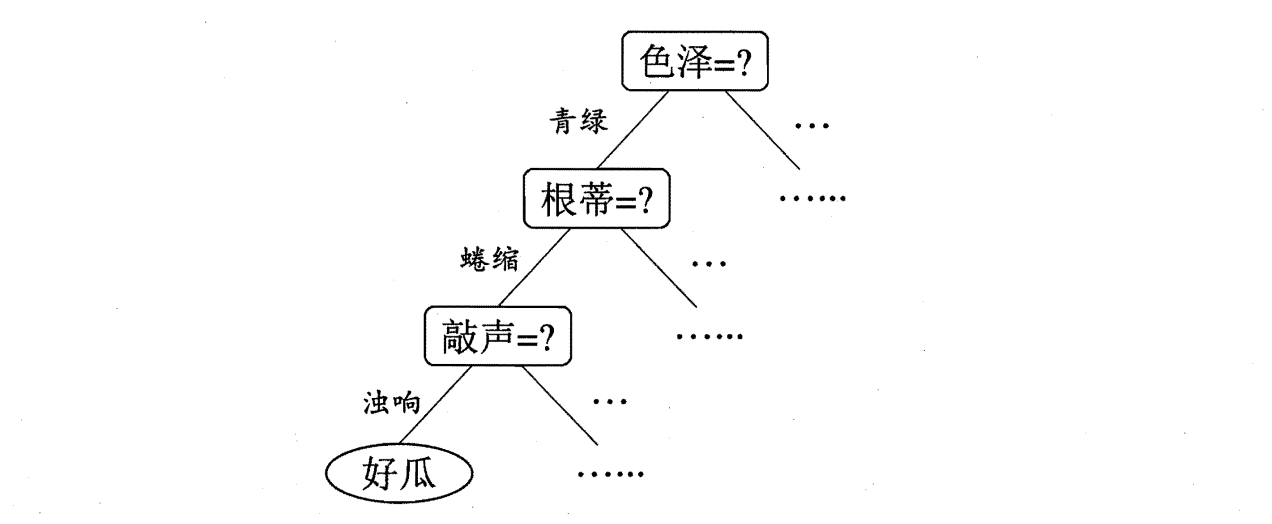
\includegraphics[width=0.8\textwidth]{../img/4-1-西瓜问题的一颗决策树.png}
    \caption{西瓜问题的一颗决策树}
    \label{fig:西瓜问题的一颗决策树}
\end{figure}

在上图的决策树中,决策过程的每一次判定都是对某一属性的“测试”,决策最终结论则对应最终的判定结果。一般的,一颗决策树包含一个根结点、若干个内部结点和若干个叶结点;叶结点对应于决策结果,其他每个结点则对应与一个属性测试;每个结点包含的样本集合根据属性测试的结果被划分到子结点中;根结点包含样本全集,从根结点到每个叶结点的路径对应了一个判定测试序列:

\begin{enumerate}[\hspace*{2em} i.]
    \item 每个非叶结点表示一个特征属性测试,叶结点对应于决策结果。
    \item 每个分支代表这个特征属性在某个值域上的输出。
    \item 每个叶子结点存放一个类别。
    \item 每个结点包含的样本集合通过属性测试被划分到子结点中,根结点包含样本全集。
\end{enumerate}

决策树学习的目的是为了产生一颗泛化能力强的决策树,其基本流程遵循简单且直观的“分而治之”(divide-and-conquer)策略:

\begin{figure}[H]
    \centering
    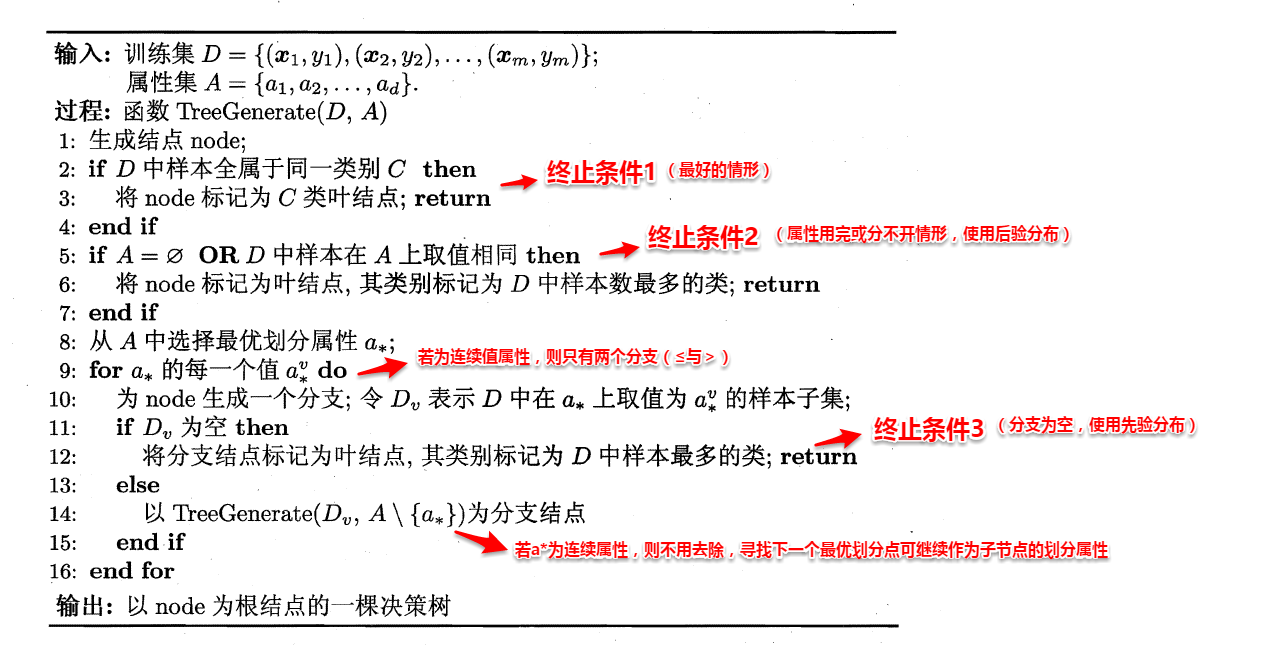
\includegraphics[width=0.8\textwidth]{../img/4-2-决策树学习基本算法.png}
    \caption{决策树学习基本算法}
    \label{fig:决策树学习基本算法}
\end{figure}

决策树的构造是一个递归的过程,有三种情形会导致递归终止:

\begin{enumerate}[\hspace*{2em} i.]
    \item 当前结点包含的样本全部属于同一类别,无需划分。
    \item 当前属性集为空,或是所有样本在所有属性上取值相同,无法划分。这时将该节点标记为叶节点,并将其类别设为该节点所含样本最多的类别。
    \item 当前结点包含的样本集和唯恐,不能划分。这时也将该节点标记为叶节点,并将其类别设为父节点中所含样本最多的类别。
\end{enumerate}

\section{划分选择}

可以看出:决策树学习的关键在于如何选择划分属性,不同的划分属性得出不同的分支结构,从而影响整颗决策树的性能。属性划分的目标是让各个划分出来的子节点尽可能地“纯”,即属于同一类别。因此下面便是介绍量化纯度的具体方法,决策树最常用的算法有三种:ID3,C4.5和CART。

\subsection{信息增益(ID3算法)}

“信息熵”(information entropy)是度量样本集合纯度最常用的一种指标。假定当前样本集合 $D$ 中第 $k$ 类样本所占的比例为 $p_k (k = 1, 2, \cdots, |Y|)$,则 $D$ 的信息熵定义为:
\begin{equation*}
    Ent(D) = - \sum_{k = 1}^{|Y|} p_k \log_2 p_k
\end{equation*}
$Ent(D)$ 的值越小,则 $D$ 的纯度越高。

假定离散属性 $a$ 有 $V$ 个可能的取值 $\{a^1, a^2, \cdots, a^V\}$,若使用 $a$ 来对样本集 $D$ 进行划分,则会产生 $V$ 个分支结点,其中第 $v$ 个分支结点包含了 $D$ 中所有在属性 $a$ 上取值为 $a^v$ 的样本,记为 $D^v$。

已知:分支结点包含的样本数越多,表示该分支结点的影响力越大,于是可计算出用属性 $a$ 对样本集 $D$ 进行划分所获得的“信息增益”(information gain):
\begin{equation*}
    Gain(D, a) = Ent(D) - \sum_{v = 1}^{V} \frac{|D^v|}{|D|} Ent(D^v)
\end{equation*}

一般而言,信息增益越大,表示使用该属性划分样本集 $D$ 的效果越好,因此在 ID3 算法在递归过程中,每次选择最大信息增益的属性作为当前的划分属性。

\subsection{增益率(C4.5算法)}

ID3 算法存在一个问题,就是偏向于取值数目较多的属性,例如:如果存在一个唯一标识,这样样本集 $D$ 将会被划分为|D|个分支,每个分支只有一个样本,这样划分后的信息熵为零,十分纯净,但是对分类毫无用处。因此C4.5算法使用了“增益率”(gain ratio)来选择划分属性,来避免这个问题带来的困扰。首先使用ID3算法计算出信息增益高于平均水平的候选属性,接着C4.5计算这些候选属性的增益率,增益率定义为:
\begin{equation*}
    Gain\_ratio(D, a) = \frac{Gain(D, a)}{IV(a)}
\end{equation*}
其中:
\begin{equation*}
    IV(a) = - \sum_{v = 1}^{V} \frac{|D^v|}{|D|} \log_2 \frac{|D^v|}{|D|}
\end{equation*}
称为属性 $a$ 的“固有值”(intrinsic value),其可能取值越多,则 $IV(a)$ 越大。

\subsection{基尼系数(CART算法)}

CART决策树使用“基尼指数”(Gini index)来选择划分属性,基尼指数反映的是从样本集 $D$ 中随机抽取两个样本,其类别标记不一致的概率,因此 $Gini(D)$ 越小越好,基尼指数定义如下:
\begin{equation*}
    Gini(D) = \sum_{k = 1}^{|Y|} \sum_{k^\prime \ne k} p_k p_{k^\prime} = 1 - \sum_{k = 1}^{|Y|} p_k^2
\end{equation*}

进而,使用属性 $a$ 划分后的基尼系数为:
\begin{equation*}
    Gini\_index(D, a) = \sum_{v = 1}^{V} \frac{|D^v|}{|D|} Gini(D^v)
\end{equation*}

\section{剪枝处理}

从决策树的构造流程中我们可以直观地看出:不管怎么样的训练集,决策树总是能很好地将各个类别分离开来,这时就会遇到之前提到过的问题:“过拟合”(overfitting),即太依赖于训练样本。剪枝(pruning)则是决策树算法对付过拟合的主要手段,剪枝的策略有两种如下:

\begin{enumerate}[\hspace*{2em} i.]
    \item “预剪枝”(prepruning):在构造的过程中先评估,再考虑是否分支。
    \item “后剪枝”(postpruning):在构造好一颗完整的决策树后,自底向上,评估分支的重要性。
\end{enumerate}

评估指的是性能度量,即决策树的泛化性能。之前提到:可以使用测试集作为学习器泛化性能的近似,因此可以将数据集划分为训练集和测试集。预剪枝表示在构造数的过程中,对一个节点考虑是否分支时,首先计算决策树不分支时在测试集上的性能,再计算分支之后的性能,若分支对性能没有提升,则选择不分支(即剪枝)。后剪枝则表示在构造好一颗完整的决策树后,从最下面的节点开始,考虑该节点分支对模型的性能是否有提升,若无则剪枝,即将该节点标记为叶子节点,类别标记为其包含样本最多的类别。

\subsection{预剪枝}

\begin{figure}[H]
    \centering
    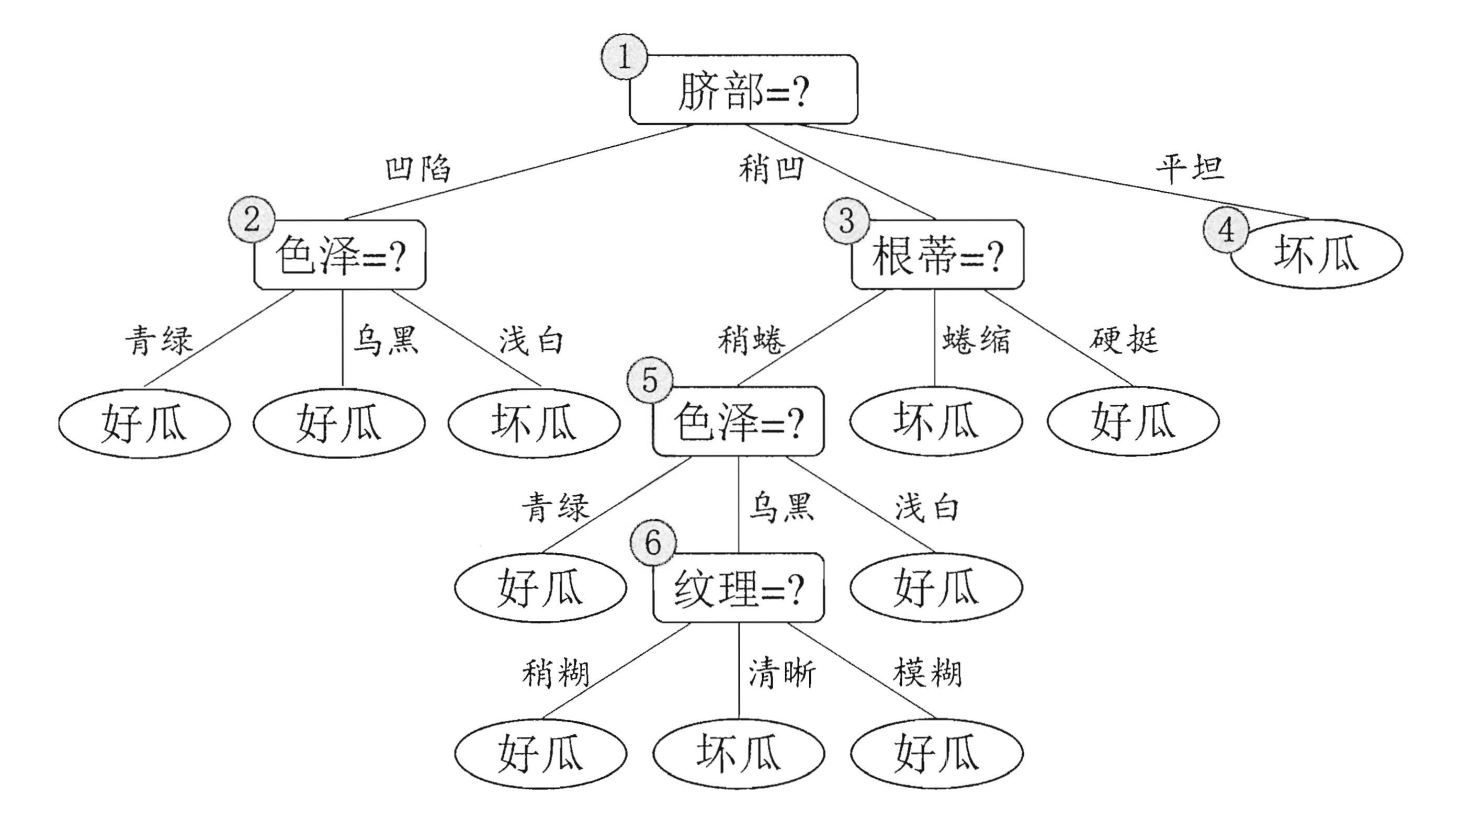
\includegraphics[width=0.8\textwidth]{../img/4-3-基于西瓜数据集2.0生成的未剪枝决策树.png}
    \caption{基于西瓜数据集2.0生成的未剪枝决策树}
    \label{fig:基于西瓜数据集2.0生成的未剪枝决策树}
\end{figure}

\begin{figure}[H]
    \centering
    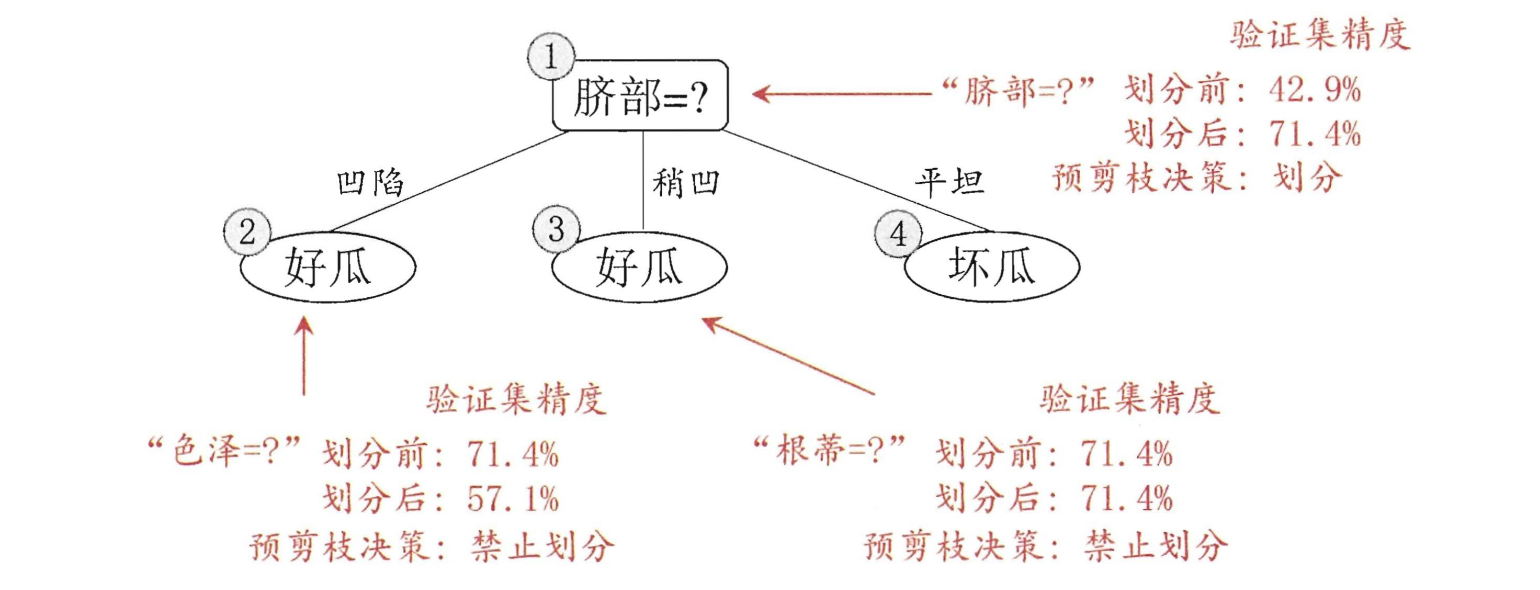
\includegraphics[width=0.8\textwidth]{../img/4-4-预剪枝决策树.png}
    \caption{预剪枝决策树}
    \label{fig:预剪枝决策树}
\end{figure}

预剪枝处理使得决策树的很多分支被剪掉,因此大大降低了训练时间开销,同时降低了过拟合的风险,但另一方面由于剪枝同时剪掉了当前节点后续子节点的分支,因此预剪枝“贪心”的本质阻止了分支的展开,在一定程度上带来了欠拟合的风险。

\subsection{后剪枝}

\begin{figure}[H]
    \centering
    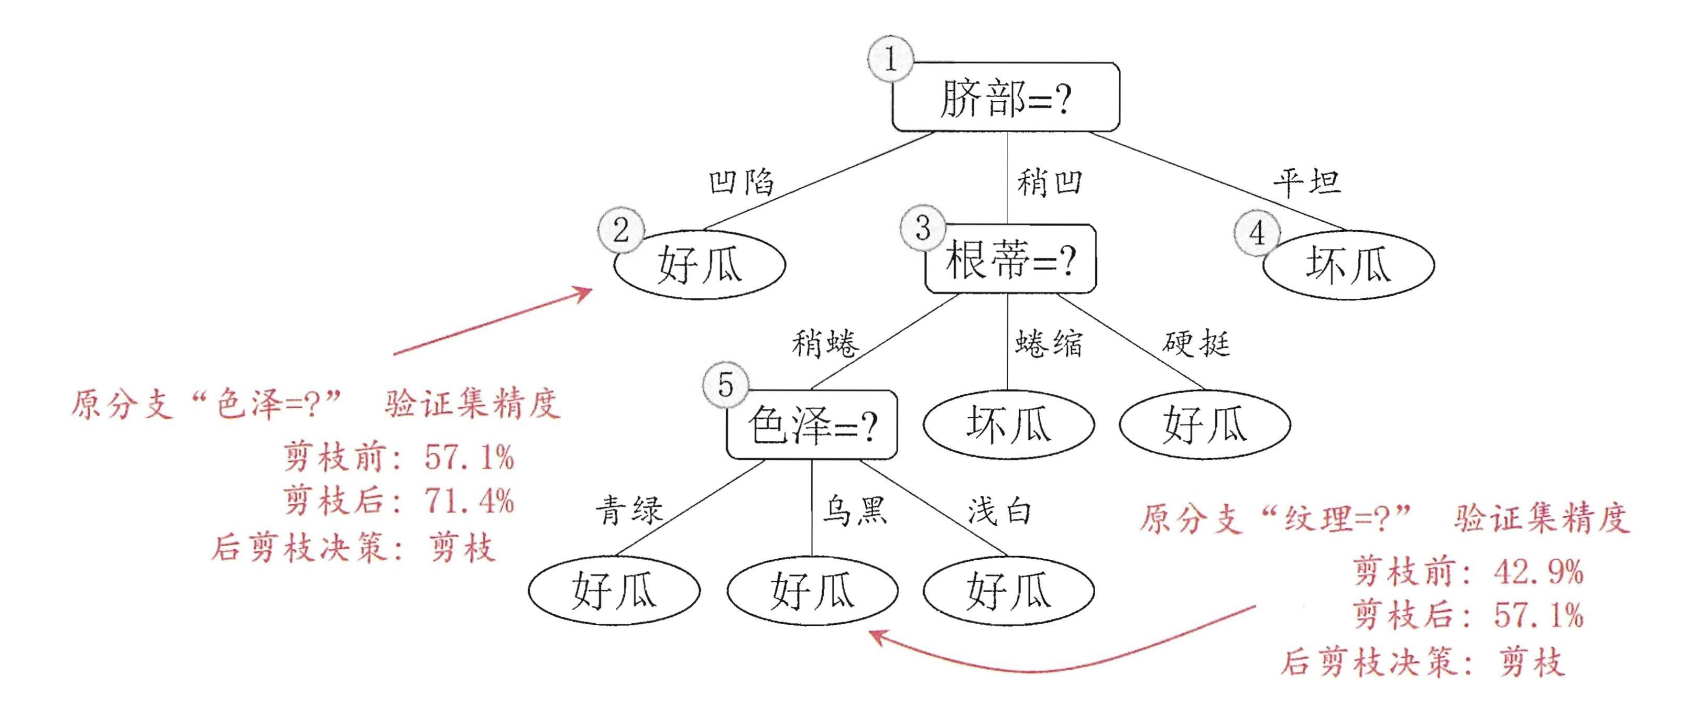
\includegraphics[width=0.8\textwidth]{../img/4-5-后剪枝决策树.png}
    \caption{后剪枝决策树}
    \label{fig:后剪枝决策树}
\end{figure}

后剪枝则通常保留了更多的分支,因此采用后剪枝策略的决策树性能往往优于预剪枝,但其自底向上遍历了所有节点,并计算性能,训练时间开销相比预剪枝大大提升。

\section{连续与缺失值}

\subsection{连续值处理}

到目前为止我们仅讨论了基于离散属性来生成决策树,现实任务中常会遇到连续属性。我们需要将连续属性进行离散化处理,常用的方法是二分法(bi-partition)。本思想为:给定样本集 $D$ 与连续属性 $a$,二分法试图找到一个划分点 $t$ 将样本集 $D$ 在属性 $a$ 上分为 $\le t$ 与 $>t$。

\begin{enumerate}[\hspace*{2em} i.]
    \item 首先将样本集 $D$ 上的连续属性 $a$ 的 $n$ 个不同取值从小到大排序,记为 $\{a^1, a^2, \cdots, a^n\}$。显然,对相邻的属性值取值 $a^i$ 与 $a^{i + 1}$ 来说,$t$ 在区间 $[a^i, a^{i + 1})$ 中取任意值所产生的划分结果相同。因此,为了便于计算,我们取均值作为划分点:
    \begin{equation*}
        T_a = \{
            \frac{a^i + a^{i + 1}}{2} | 1 \le i \le n - 1
        \}
    \end{equation*}
    \item 计算每一个划分点划分集合 $D$ 后的信息增益。
    \item 选择最大信息增益的划分点作为最优划分点。
    \begin{equation*}
        Gain(D, a) = \max_{t \in T_a} Gain(D, a, t) = \max_{t \in T_a} Ent(D) - \sum_{\lambda \in \{-, +\}} \frac{|D_t^\lambda|}{|D|} Ent(D_t^\lambda)
    \end{equation*}
\end{enumerate}

\subsection{缺失值处理}

现实中常会遇到不完整的样本,即某些属性值缺失。有时若简单采取剔除,则会造成大量的信息浪费,因此在属性值缺失的情况下需要解决两个问题:

\begin{enumerate}[\hspace*{2em} i.]
    \item 如何选择划分属性。
    \item 给定划分属性,若某样本在该属性上缺失值,如何划分到具体的分支上。
\end{enumerate}

假定为样本集中的每一个样本都赋予一个权重,根节点中的权重初始化为 $1$,则定义:

样本子集所占比例:
\begin{equation*}
    \rho = \frac{\sum_{x \in \tilde{D}} w_x}{\sum_{x \in D} w_x}
\end{equation*}

样本子集每个类别的比例:
\begin{equation*}
    \tilde{p}_k = \frac{\sum_{x \in \tilde{D}_k} w_x}{\sum_{x \in \tilde{D}} w_x}, \ \ \ 1 \le k \le |Y|
\end{equation*}

每个分支所含样本比例:
\begin{equation*}
    \tilde{r}_v = \frac{\sum_{x \in \tilde{D}^v} w_x}{\sum_{x \in D} w_x}, \ \ \ 1 \le v \le V
\end{equation*}

对于问题 $1$:通过在样本集 $D$ 中选取在属性 $a$ 上没有缺失值的样本子集,计算在该样本子集上的信息增益,最终的信息增益等于该样本子集划分后信息增益乘以样本子集占样本集的比重。即:
\begin{equation*}
    Gain(D, a) = \rho \times Gain(\tilde{D}, a) = \rho \times \left(
        Ent (\tilde{D}) - \sum_{v = 1}^{V} \tilde{r}_v Ent (\tilde{D}^v)
    \right)
\end{equation*}
其中:
\begin{equation*}
    Ent(\tilde{D}) = - \sum_{k = 1}^{|Y|} \tilde{p}_k \log_2 \tilde{p}_k
\end{equation*}

对于问题 $2$:若该样本子集在属性 $a$ 上的值缺失,则将该样本以不同的权重(即每个分支所含样本比例)划入到所有分支节点中。该样本在分支节点中的权重变为:
\begin{equation*}
    w_x = w_x \cdot \tilde{r}_v
\end{equation*}




\end{document}